\section{Results}


\begin{table*}[t]
	\footnotesize
	\centering
	\caption{Effectiveness of LLM-generated Boolean queries on the PubTemp set. \textbf{Bold} indicates the best result for each model within a setting; \underline{Underlined} indicates the overall best across all models. (O3 model has no N.R capability as reasoning was enabled by default using API.~\vspace{-9pt})}
	\label{tab:eval-results-pubmed}
		\begin{tabular*}{\textwidth}{@{\extracolsep{\fill}}lllllllllll@{}}
			\toprule
			%\multicolumn{3}{c}{} & \multicolumn{4}{c}{\textbf{Primary Metrics}} & \multicolumn{4}{c}{\textbf{Secondary Metrics}} \\
			\cmidrule(lr){4-7} \cmidrule(lr){8-11}
			Setting & Model & Prompt & Recall & F3 & \parbox{2.5em}{Recall\\>80\%} & \parbox{2.5em}{Recall\\>90\%} & Precision & \parbox{4em}{Avg\\Retrieved} & \parbox{2.5em}{Avg\\Regen} & \%Success \\
			\midrule
			\multirow{11}{*}{\rotatebox{90}{Zero-shot}} & GPT-4o & N.R & 0.3591 & \textbf{0.1758} & 12.40 & 7.10 & \underline{\textbf{0.1074}} & \textbf{251.32} & 1.15 & 99.60 \\
			& GPT-4o & R & 0.3937 & 0.1653 & 14.30 & 9.00 & 0.0913 & 326.20 & 1.09 & 99.80 \\
			& GPT-4o & R-con & \textbf{0.4387} & 0.1491 & \textbf{15.90} & \textbf{9.40} & 0.0642 & 440.45 & \underline{\textbf{1.04}} & \textbf{99.90} \\
			& GPT-4o & R-obj & 0.2530 & 0.0988 & 5.30 & 3.10 & 0.0742 & 359.00 & 1.20 & 99.80 \\
			\cmidrule{3-11}
			& O3 & R & \textbf{0.6868} & 0.2039 & \textbf{44.80} & \textbf{31.80} & 0.0611 & 551.54 & 1.69 & 98.20 \\
			& O3 & R-con & 0.6483 & \underline{\textbf{0.2106}} & 38.60 & 26.20 & \textbf{0.0690} & \textbf{499.48} & \textbf{1.19} & 99.70 \\
			& O3 & R-obj & 0.5153 & 0.1293 & 22.70 & 14.70 & 0.0510 & 603.10 & 1.21 & \underline{\textbf{100.00}} \\
			\cmidrule{3-11}
			& Qwen3-4B & N.R & 0.0098 & 0.0074 & 0.00 & 0.00 & 0.0175 & \underline{\textbf{64.72}} & 7.93 & 25.60 \\
			& Qwen3-4B & R & 0.0681 & 0.0429 & 0.70 & 0.60 & \textbf{0.0640} & 105.13 & 3.86 & 84.40 \\
			& Qwen3-4B & R-con & \textbf{0.3458} & \textbf{0.0824} & \textbf{11.60} & \textbf{6.50} & 0.0402 & 514.11 & \textbf{1.29} & \textbf{99.60} \\
			& Qwen3-4B & R-obj & 0.0676 & 0.0212 & 1.40 & 1.10 & 0.0233 & 306.53 & 2.89 & 93.80 \\
			\midrule
			\multirow{4}{*}{\rotatebox{90}{\shortstack{AutoBool \\ ($\alpha = 0.5$) \\ Weak R.O}}} & Qwen3-4B & N.R & \textbf{0.6791} & \textbf{0.1386} & \textbf{42.70} & \textbf{30.80} & \textbf{0.0392} & 677.31 & 1.12 & 98.80 \\
			& Qwen3-4B & R & 0.6112 & 0.1223 & 33.60 & 21.70 & 0.0345 & 678.80 & \underline{\textbf{1.04}} & 99.60 \\
			& Qwen3-4B & R-con & 0.5202 & 0.1052 & 22.80 & 14.30 & 0.0388 & \textbf{654.57} & 1.11 & \textbf{99.80} \\
			& Qwen3-4B & R-obj & 0.6495 & 0.0987 & 39.10 & 25.50 & 0.0263 & 743.89 & 1.10 & 99.40 \\
			\midrule
			\multirow{4}{*}{\rotatebox{90}{\shortstack{AutoBool \\ ($\alpha = 1$) \\ Mod R.O}}} & Qwen3-4B & N.R & \underline{\textbf{0.7036}} & 0.1195 & \underline{\textbf{47.10}} & \underline{\textbf{32.30}} & 0.0300 & 732.49 & 1.17 & 98.40 \\
			& Qwen3-4B & R & 0.5453 & \textbf{0.1346} & 27.90 & 16.50 & \textbf{0.0496} & \textbf{586.01} & 1.06 & 99.70 \\
			& Qwen3-4B & R-con & 0.5262 & 0.1066 & 26.30 & 16.80 & 0.0372 & 636.19 & 1.06 & \underline{\textbf{100.00}} \\
			& Qwen3-4B & R-obj & 0.6540 & 0.1094 & 39.70 & 26.70 & 0.0293 & 738.34 & \underline{\textbf{1.04}} & 99.90 \\
			\midrule
			\multirow{4}{*}{\rotatebox{90}{\shortstack{AutoBool \\ ($\alpha = 2$) \\ Heavy R.O}}} & Qwen3-4B & N.R & \textbf{0.6948} & 0.1209 & \textbf{45.30} & 30.80 & 0.0306 & 724.15 & 1.11 & 98.90 \\
			& Qwen3-4B & R & 0.5602 & \textbf{0.1344} & 30.00 & 18.40 & \textbf{0.0472} & \textbf{588.21} & 1.07 & 99.60 \\
			& Qwen3-4B & R-con & 0.5911 & 0.0887 & 31.40 & 20.40 & 0.0281 & 739.69 & 1.09 & \textbf{99.80} \\
			& Qwen3-4B & R-obj & 0.6878 & 0.1024 & 44.80 & \textbf{31.30} & 0.0245 & 773.01 & \textbf{1.06} & 99.70 \\
			\bottomrule
			
		\end{tabular*}
		~\vspace{-12pt}
\end{table*}






















Table~\ref{tab:eval-results-pubmed} summarizes the evaluation results on the PubTemp set. We observe that reinforcement learning substantially improves Boolean query generation performance, especially in recall-critical settings like systematic reviews. 

\subsection{Effectiveness of Reinforcement Learning}
Compared to zero-shot prompting baselines using the same base model (Qwen3-4B), all RL-trained AutoBool models achieve substantially higher effectiveness. Top models obtain 0.70 average recall, with 35\% of queries exceeding 90\% recall, versus 0.35 recall and 6.5\% for zero-shot baselines. We also compare against in-context learning (ICL) with 1-shot, 3-shot, and 5-shot configurations (Appendix~\ref{appendix:icl}): AutoBool achieves 7× improvement over the best ICL result, demonstrating that RL provides optimization signals that cannot be communicated through examples alone.

On secondary metrics, AutoBool models improve precision under the \texttt{N.R} and \texttt{R-obj} prompts, but slightly reduce precision under \texttt{R} and \texttt{R-con}. All trained models retrieve more documents than their zero-shot counterparts: an expected trade-off when optimizing for recall. However, this increase in retrieved set size remains reasonable (well under 1000 on average), and does not significantly increase screening burden compared to the gains in comprehensiveness.


Training also improves generation stability. AutoBool models exhibit consistently higher success rates (near 100\%) and require fewer regenerations than zero-shot baselines, indicating more reliable formatting and syntactic validity—driven by our structured reward components.

\paragraph{Comparison with Larger GPT-Based Models.}
Compared to significantly larger GPT-based models (GPT-4o and O3),%
~\footnote{While parameter counts are proprietary, these models are widely estimated to be ~100× larger than our 4B backbone.}
AutoBool, despite using a much smaller model, achieves higher recall and a higher percentage of queries exceeding high-recall thresholds (e.g., 80\% and 90\%). Regeneration and success rates are also comparable across models. While AutoBool has lower precision and F\textsubscript{3}, this reflects domain-specific optimization: the screening burden difference is modest (O3: 499--603 documents vs AutoBool: 586--773), representing only 5–6 additional hours in a 30+ hour process, while missing studies can invalidate entire reviews. The average number of retrieved documents remains within a practical range, and AutoBool enables local deployment for organizations with API privacy restrictions. These results highlight the effectiveness of retrieval-driven RL training in generating high-recall Boolean queries, even under constrained model capacity.


\paragraph{Effect of Prompt Type.}
Under zero-shot settings, the \texttt{R-con} prompt generally yields the highest recall and F\textsubscript{3} scores (except for F\textsubscript{3} in GPT-4o and recall in O3), suggesting that structured reasoning aids query formulation when no retrieval feedback is available. However, this advantage diminishes after training. For trained AutoBool models, the \texttt{No Reasoning} prompt consistently achieves the best recall and high-recall threshold performance across all settings, while reasoning-based prompts tend to yield higher precision.

We hypothesize two complementary explanations for these trends. First, RL enables the model to internalize task-specific structure and discover its own optimized generation strategy, which may diverge from human-designed decomposition frameworks. Second, Boolean queries are inherently interpretable and self-contained: their logic is fully encoded through syntax and operators. As such, requiring the model to verbalize intermediate reasoning may introduce unnecessary constraints or verbosity once it has learned to generate effective queries end-to-end.

Nonetheless, reasoning-based prompts consistently yield higher success rates and require fewer regenerations than \texttt{No Reasoning}, even after training. This suggests that intermediate reasoning may still offer robustness benefits in more difficult systematic review topics, where generating a valid and well-formed Boolean query is especially challenging. In these cases, explicit reasoning may help the model maintain syntactic and semantic integrity under ambiguity or complexity.


\paragraph{Which \texorpdfstring{$\alpha$}{α} Value Should Be Used?}
We analyze the effect of the \(\alpha\) parameter in the retrieval reward, which adjusts the emphasis on recall over precision. In structured reasoning-based prompts (\texttt{R-con}, \texttt{R-obj}), increasing \(\alpha\) consistently improves recall, as intended. In contrast, results are more mixed for less-structured prompts: \(\alpha = 1\) yields the highest recall with \texttt{N.R}, while \(\alpha = 0.5\) performs best with \texttt{R}. For F\textsubscript{3}, \(\alpha = 1\) generally achieves the best performance across prompts, except in \texttt{N.R}, where \(\alpha = 0.5\) outperforms. Overall, \(\alpha = 1\) offers the most balanced trade-off between recall and precision, making it a strong default. Its effects are also more stable in structured prompts, where recall improves more predictably with higher \(\alpha\).


\begin{figure*}[htbp]
	\centering
	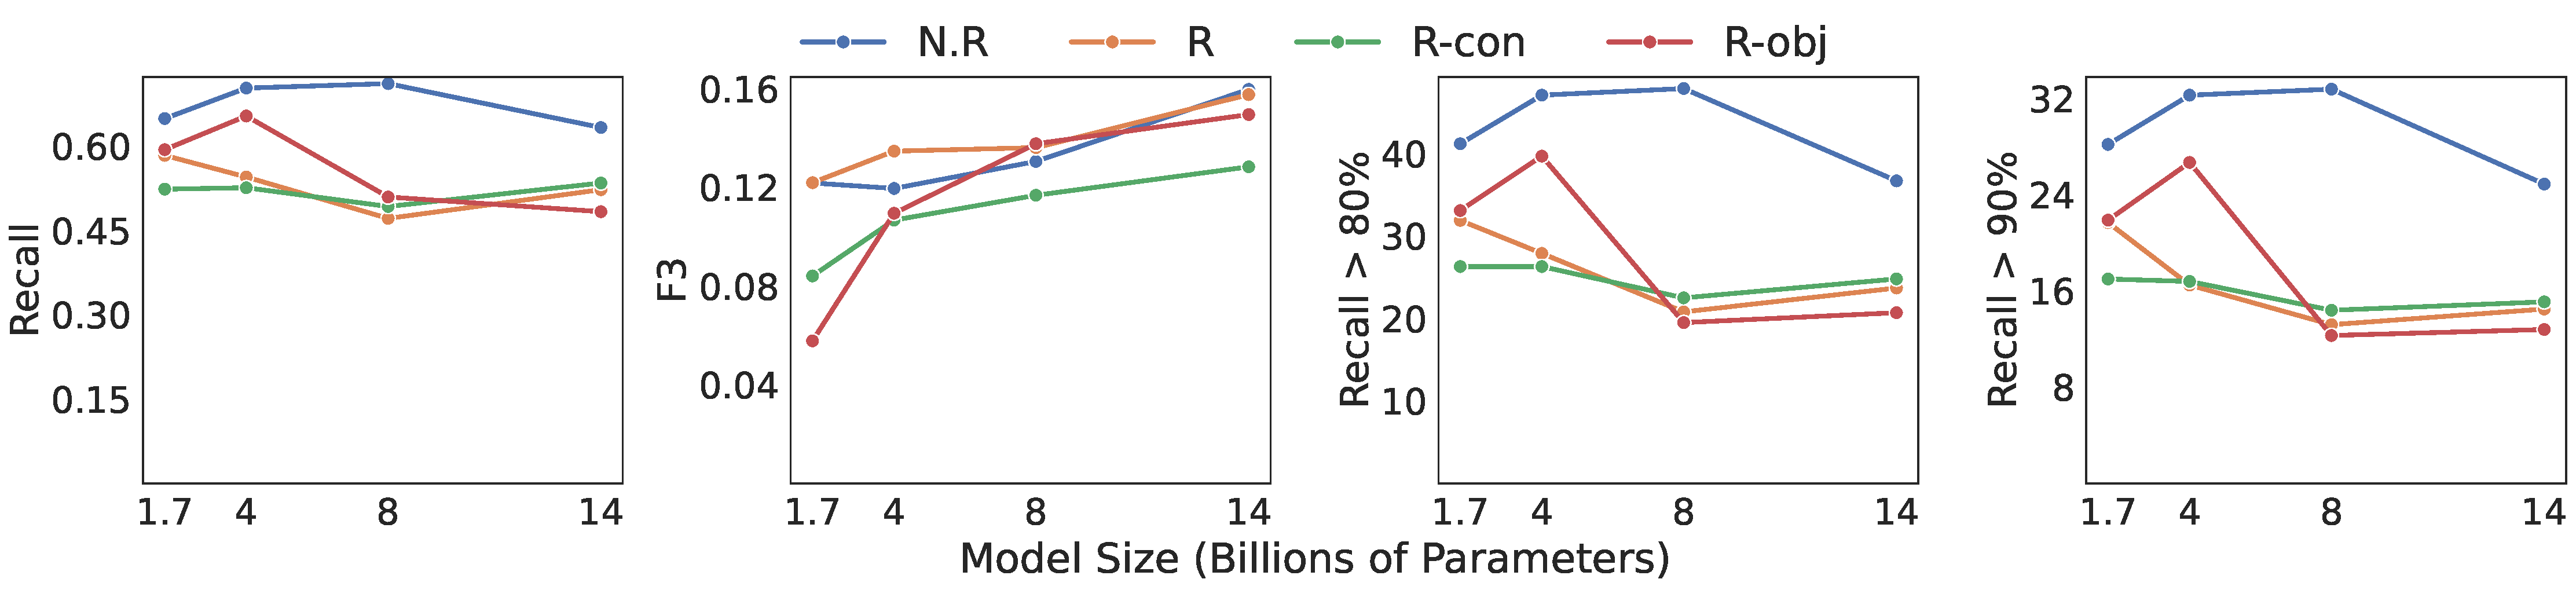
\includegraphics[width=\textwidth]{figures/trained_model_size_comparison_final.pdf}
	\caption{Effect of model size on the effectiveness of Boolean query generation across prompt types on the PubMed Temporal-Cutoff set, all result based on Qwen3 based Models.}
		\label{fig:model-size-comparison}
\end{figure*}

\subsubsection{Generalization on Existing Datasets}

To assess generalization, we evaluate our trained models on two established systematic review benchmarks: CLEF TAR and the Seed Collection (Table~\ref{tab:eval-results-clef} and Table~\ref{tab:eval-results-seed} in Appendix). Both datasets are relatively small and publicly available, raising potential concerns around bias and data leakage.

\textbf{For CLEF TAR,} AutoBool generalizes well, obtaining substantially higher recall and recall-threshold metrics than its zero-shot counterparts. It is also more effective than larger models like GPT-4o and O3 in recall. With \(\alpha = 1\) and the \texttt{No Reasoning} prompt, AutoBool almost matches the recall of expert-crafted queries (within 1\%) while retrieving 17 times fewer documents; yielding improved F\textsubscript{3}, higher precision, and reduced screening effort. It is also more effective than the O1 model from~\citet{wang2025reassessing} in both recall and F\textsubscript{3}, highlighting the benefits of RL optimization.
\textbf{For Seed Collection,} a similar pattern holds. While AutoBool is less effective than expert-written queries, it is significantly more effective than zero-shot baselines and the O1 model from~\citet{wang2025reassessing}. These results demonstrate that retrieval-aware training enables robust Boolean query generation, even when trained on a single corpus.


